\documentclass[bigtut]{tutorial}\usepackage[]{graphicx}\usepackage[]{color}
%% maxwidth is the original width if it is less than linewidth
%% otherwise use linewidth (to make sure the graphics do not exceed the margin)
\makeatletter
\def\maxwidth{ %
  \ifdim\Gin@nat@width>\linewidth
    \linewidth
  \else
    \Gin@nat@width
  \fi
}
\makeatother

\definecolor{fgcolor}{rgb}{0.345, 0.345, 0.345}
\newcommand{\hlnum}[1]{\textcolor[rgb]{0.686,0.059,0.569}{#1}}%
\newcommand{\hlstr}[1]{\textcolor[rgb]{0.192,0.494,0.8}{#1}}%
\newcommand{\hlcom}[1]{\textcolor[rgb]{0.678,0.584,0.686}{\textit{#1}}}%
\newcommand{\hlopt}[1]{\textcolor[rgb]{0,0,0}{#1}}%
\newcommand{\hlstd}[1]{\textcolor[rgb]{0.345,0.345,0.345}{#1}}%
\newcommand{\hlkwa}[1]{\textcolor[rgb]{0.161,0.373,0.58}{\textbf{#1}}}%
\newcommand{\hlkwb}[1]{\textcolor[rgb]{0.69,0.353,0.396}{#1}}%
\newcommand{\hlkwc}[1]{\textcolor[rgb]{0.333,0.667,0.333}{#1}}%
\newcommand{\hlkwd}[1]{\textcolor[rgb]{0.737,0.353,0.396}{\textbf{#1}}}%

\usepackage{framed}
\makeatletter
\newenvironment{kframe}{%
 \def\at@end@of@kframe{}%
 \ifinner\ifhmode%
  \def\at@end@of@kframe{\end{minipage}}%
  \begin{minipage}{\columnwidth}%
 \fi\fi%
 \def\FrameCommand##1{\hskip\@totalleftmargin \hskip-\fboxsep
 \colorbox{shadecolor}{##1}\hskip-\fboxsep
     % There is no \\@totalrightmargin, so:
     \hskip-\linewidth \hskip-\@totalleftmargin \hskip\columnwidth}%
 \MakeFramed {\advance\hsize-\width
   \@totalleftmargin\z@ \linewidth\hsize
   \@setminipage}}%
 {\par\unskip\endMakeFramed%
 \at@end@of@kframe}
\makeatother

\definecolor{shadecolor}{rgb}{.97, .97, .97}
\definecolor{messagecolor}{rgb}{0, 0, 0}
\definecolor{warningcolor}{rgb}{1, 0, 1}
\definecolor{errorcolor}{rgb}{1, 0, 0}
\newenvironment{knitrout}{}{} % an empty environment to be redefined in TeX

\usepackage{alltt}
\usepackage{amsmath}      % for boxes
\unitcode{MATH1005}
        \unitname{Statistics}
        \semester{Summer/Winter/Semester2}
        \sheetnumber3

\usepackage{graphicx}
%\withsolutions
\IfFileExists{upquote.sty}{\usepackage{upquote}}{}
\begin{document}
\lettersfirst

\begin{tutorial}

\begin{center}
\begin{tabular}{| ll | } \hline
& \\
{\bf Numerical Summaries} & \\
Given a sample $\{x_i\}$ and ordered data $\{ x_{(i)} \} $ &  for $i=1,\ldots,n$ \\   
& \\
sample mean &  $\bar x = \frac{1}{n} \sum_{i=1}^n x_i$    \\ 
sample variance &  $s^2=  \frac{1}{n-1} \sum_{i=1}^n (x_i - \bar x)^2 
= \frac1{n-1}\left( \sum_{i=1}^n x_i^2 - \frac{1}{n}\Bigl(\sum_ {i=1}^n x_i\Bigr)^2\right)$ \\
&  $= \frac1{n-1}\left( \sum_{i=1}^n x_i^2 -  n \bar{x}^2  \right)$   \\
%sample standard deviation &  $s=   \sqrt{ \frac{1}{n-1} \sum_{i=1}^n (x_i - \bar x)^2 } 
sample standard deviation &  $s$  \\
 %=  \sqrt{ \frac1{n-1}\left( \sum_{i=1}^n x_i^2 -  n \bar{x}^2  \right)} $  
%Median (or 2nd Quartile) & $\tilde{x} =Q_{2} =  \frac{ x_{  ( \lceil \frac{n+1}{2}  \rceil )  } + x_{ ( \lfloor \frac{n+1}{2} \rfloor  )  }   }{2}$ \\
Median (or 2nd Quartile) & $\tilde{x} =Q_{2} =  \mbox{Middle data point in sorted data}$ (for $n$ odd) \\
 & and Average of 2 middle sorted data points (for $n$ even) \\
%1st quartile &  $Q_{1}=  \frac{ x_{ (\lceil     \frac{n}{4}  \rceil      )  } + x_{ ( \lfloor   \frac{n}{4} +1  \rfloor    ) }}{2}$ \\
1st quartile &  $Q_{1}=  \mbox{Median of bottom half of sorted data}$  \\
3rd quartile &  $Q_{3}=  \mbox{Median of top half of sorted data}$ \\

%3rd quartile & $Q_{3} =  \frac{ x_{ ( \lceil   \frac{3n}{4}  \rceil  )  } + x_{ (   \lfloor   \frac{3n}{4} +1  \rfloor    )     }}{2}$ \\
Five number summary & ($x_{(1)}$, $Q_{1}$, $Q_{2}$, $Q_{3}$, $x_{(n)}$) \\ 
Interquartile Range & $IQR = Q_{3} - Q_{1}$ \\
Boxplot Thresholds (for outliers) & $LT = Q_{1} - 1.5 IQR$, $UT = Q_{3} + 1.5 IQR$ \\
& \\ \hline
\end{tabular}
\end{center}

Note:  \\
(1) There are 3 formulae for the variance: the 1st one is the definition formula and the others are calculation formulae. \\
(2) For calculating $Q_{1}$ and $Q_{3}$, we include the median in each half set (when $n$ is odd).


\vspace{.5cm}
\begin{questions}

\question Australian Road Fatalities \& Australian Commercial Refrigerators

\begin{knitrout}
\definecolor{shadecolor}{rgb}{0.969, 0.969, 0.969}\color{fgcolor}\begin{kframe}
\begin{alltt}
\hlstd{Road} \hlkwb{<-} \hlkwd{read.csv}\hlstd{(}\hlstr{"http://www.maths.usyd.edu.au/u/UG/JM/MATH1005/r/StatsData/
                 AllFatalities.csv"}\hlstd{)}
\hlstd{Age} \hlkwb{<-} \hlstd{Road}\hlopt{$}\hlstd{Age}
\hlstd{AgeN}\hlkwb{<-} \hlkwd{as.numeric}\hlstd{(}\hlkwd{levels}\hlstd{(Age))[Age]}
\hlkwd{class}\hlstd{(AgeN)}
\hlkwd{fivenum}\hlstd{(AgeN)} \hlcom{#To get quartiles}
\hlkwd{summary}\hlstd{(AgeN)}  \hlcom{#To get mean}
\hlkwd{boxplot}\hlstd{(AgeN)}
\end{alltt}
\end{kframe}
\end{knitrout}

\begin{knitrout}
\definecolor{shadecolor}{rgb}{0.969, 0.969, 0.969}\color{fgcolor}\begin{kframe}
\begin{alltt}
\hlstd{Fridge} \hlkwb{<-} \hlkwd{read.csv}\hlstd{(}\hlstr{"http://www.maths.usyd.edu.au/u/UG/JM/MATH1005/r/StatsData/
                 Refrigerators.csv"}\hlstd{)}
\hlstd{Efficiency} \hlkwb{<-} \hlstd{Fridge}\hlopt{$}\hlstd{Efficiency..kWh.24h.m..}
\hlkwd{fivenum}\hlstd{(Efficiency)}
\hlkwd{mean}\hlstd{(Efficiency)}
\hlkwd{median}\hlstd{(Efficiency)}
\end{alltt}
\end{kframe}
\end{knitrout}

\vspace{.5cm}
For the both Age and Efficiency, what is the mean and median? Which one would you report and why?

\begin{solution}
As both data sets show some skewing, the median (robust) would be preferable, especially with Efficiency which has outliers.
\end{solution}

%\newpage for Solutions
\question Sigma Notation and Numerical Summaries \\

For each part, work out the answers by hand and then check in R. \\

\begin{parts}
\part 
Given the data $x=\{ 1, 2, 3, 6, 7, 9 \}$ and $y=\{ 1, 1, 2, 3, 4, 4 \}$, calculate 
\begin{center}
$\sum_{i=1}^{6} x_i$ \hspace{.5cm}
$\sum_{i=1}^{6} x_i^2$ \hspace{.5cm}
$\sum_{i=1}^6 x_i y_i $ \hspace{.5cm} 
$\sum_{i=1}^3(x_i-5)^2$ \hspace{.5cm}
$\sum_{i=2}^3 y_{(i)}^2$ \hspace{.5cm}
\end{center}

\begin{knitrout}
\definecolor{shadecolor}{rgb}{0.969, 0.969, 0.969}\color{fgcolor}\begin{kframe}
\begin{alltt}
\hlstd{x}\hlkwb{=}\hlkwd{c}\hlstd{(}\hlnum{1}\hlstd{,}\hlnum{2}\hlstd{,}\hlnum{3}\hlstd{,}\hlnum{6}\hlstd{,}\hlnum{7}\hlstd{,}\hlnum{9}\hlstd{)}
\hlstd{y}\hlkwb{=}\hlkwd{c}\hlstd{(}\hlnum{1}\hlstd{,}\hlnum{1}\hlstd{,}\hlnum{2}\hlstd{,}\hlnum{3}\hlstd{,}\hlnum{4}\hlstd{,}\hlnum{4}\hlstd{)}
\hlkwd{sum}\hlstd{(x)}
\hlkwd{sum}\hlstd{(x}\hlopt{^}\hlnum{2}\hlstd{)}
\hlkwd{sum}\hlstd{(x}\hlopt{*}\hlstd{y)}
\hlkwd{sum}\hlstd{(((x}\hlopt{-}\hlnum{5}\hlstd{)}\hlopt{^}\hlnum{2}\hlstd{)[}\hlnum{1}\hlopt{:}\hlnum{3}\hlstd{])}
\hlkwd{sum}\hlstd{((}\hlkwd{sort}\hlstd{(y)}\hlopt{^}\hlnum{2}\hlstd{)[}\hlnum{2}\hlopt{:}\hlnum{3}\hlstd{])}
\end{alltt}
\end{kframe}
\end{knitrout}

\vspace{.5cm}
\part Calculate the mean and standard deviation of $x$.

\begin{knitrout}
\definecolor{shadecolor}{rgb}{0.969, 0.969, 0.969}\color{fgcolor}\begin{kframe}
\begin{alltt}
\hlkwd{mean}\hlstd{(x)}
\hlkwd{sd}\hlstd{(x)}
\end{alltt}
\end{kframe}
\end{knitrout}

\vspace{.5cm}
\part  If each data point in $x$ is increased by 1, how would the mean and standard deviation change? Why?  Check numerically.

\begin{knitrout}
\definecolor{shadecolor}{rgb}{0.969, 0.969, 0.969}\color{fgcolor}\begin{kframe}
\begin{alltt}
\hlstd{m}\hlkwb{=}\hlstd{x}\hlopt{+}\hlnum{1}
\hlkwd{mean}\hlstd{(m)}
\hlkwd{sd}\hlstd{(m)}
\end{alltt}
\end{kframe}
\end{knitrout}

\vspace{.5cm}
\part   Find  the quartiles of $x$.

\begin{knitrout}
\definecolor{shadecolor}{rgb}{0.969, 0.969, 0.969}\color{fgcolor}\begin{kframe}
\begin{alltt}
\hlkwd{median}\hlstd{(x)}
\hlkwd{fivenum}\hlstd{(x)}
\end{alltt}
\end{kframe}
\end{knitrout}

\vspace{.5cm}
\part (Extension: This is not examinable. Just for students who want to challenge themselves.) \\
Given $m_{i} = x_{i} + 1$, show algebraically that $\bar{m} = \bar{x} + 1$ and $s_{m}^2 = s_{x}^2$.

\end{parts}

\vspace{.5cm}
\begin{solution}
\vspace{-.34cm}
(a) \\
$\sum_{i=1}^{6} x_i = 1 + 2 + \ldots 9 = 28 $. \\
$\sum_{i=1}^{6} x_i^2 = 1^2 + 2^2 + \ldots 9^2 = 180 $. \\
$\sum_{i=1}^6 x_i y_i = 1 \times 1 + 2 \times 1 + \ldots 9 \times 4 = 91$. \\
$\sum_{i=1}^3(x_i-5)^2 = (1-5)^2 + (2-5)^2 + (3-5)^2 = 29 $. \\
$\sum_{i=2}^3 y_{(i)}^2 = 1^2 + 2^2 = 5$, as $\{ y_{(i)} \} = \{ y_{i} \}$ as the data is already sorted.

Note: If say $\{ y_{i} \} = \{ 8,1,4 \}$, then $\{ y_{(i)} \} = \{ 1,4,8 \}$, so $\sum_{i=2}^3 y_{(i)}^2 = 4^2 + 8^2 = 80$. 

\vspace{.5cm}
(b) \\
$\bar{x} = \frac{1}{6} \sum_{i=1}^{6} x_{i} = \frac{28}{6} \approx 4.67 $ \\
$s= \sqrt { \frac1{5}\left( \sum_{i=1}^6 x_i^2 - \frac{1}{6} \Bigl(\sum_ {i=1}^6 x_i\Bigr)^2\right) } = \sqrt { \frac1{5}\left( 180 - \frac{1}{6} (28)^2 \right) } \approx 3.14$ 


\vspace{.5cm}
(c) \\
Mean: Increases by 1 (as the full data set shifts up by 1, the average shifts up by 1). \\
Standard deviation: Unchanged  ((as the full data set shifts up by 1, the spread is unchanged). \\

Check numerically: \\
Given $\{ m_{i} \}  = \{ x_{i} + 1 \} = \{ 2,3,4,7,8,10 \}$, then $\bar{m} \approx 5.67$ and
$s_{m}^2 \approx 3.14$.  \\

The standard deviation could also be found (the long way) in R by using the formula:
\begin{knitrout}
\definecolor{shadecolor}{rgb}{0.969, 0.969, 0.969}\color{fgcolor}\begin{kframe}
\begin{alltt}
\hlkwd{sqrt}\hlstd{(} \hlnum{1}\hlopt{/}\hlnum{5}\hlopt{*}\hlstd{(}\hlkwd{sum}\hlstd{(x}\hlopt{^}\hlnum{2}\hlstd{)} \hlopt{-} \hlnum{1}\hlopt{/}\hlnum{6}\hlopt{*}\hlkwd{sum}\hlstd{(x)}\hlopt{^}\hlnum{2}\hlstd{) )}
\hlkwd{sqrt}\hlstd{(} \hlnum{1}\hlopt{/}\hlnum{5}\hlopt{*}\hlstd{(}\hlkwd{sum}\hlstd{(x}\hlopt{^}\hlnum{2}\hlstd{)} \hlopt{-} \hlnum{6}\hlopt{*}\hlkwd{mean}\hlstd{(x)}\hlopt{^}\hlnum{2}\hlstd{) )}
\end{alltt}
\end{kframe}
\end{knitrout}

\vspace{.5cm}
(d) \\
Sorted data is $\{ x_{(i)} \} = \{ 1,2,3,6,7,9 \}$, so $\tilde{x} = \frac{3+6}{2} = 4.5$. \\
Bottom half of sorted data is: $\{ 1,2,3 \}$, so $Q_{1}=2$. \\
Top half of sorted data is: $\{ 6,7,9 \}$, so $Q_{3}=7$. \\

\vspace{.5cm}
(e) \\
If $m_{i} = x_{i} + 1$ then: \\
 $\bar{m} = \frac{1}{n} \sum_{i=1}^{n}  ( x_{i} + 1 ) = \frac{1}{n} \sum_{i=1}^{n}   x_{i} + \frac{1}{n} \sum_{i=1}^{n}  1 = \bar{x} + 1$. \\
$s_{m}^2 = \frac{1}{n-1} \sum_{i=1}^{n}  ( m_{i} -\bar{m} )^2 = \frac{1}{n-1} \sum_{i=1}^{n}  ( (x_{i}+1) -(\bar{x}+1) )^2
= \frac{1}{n-1} \sum_{i=1}^{n}  ( x_{i} -\bar{x} )^2 = s_{x}^2$.

\end{solution}


\vspace{.5cm}
\question Numerical Summaries  \\

A sample of 36 mice was used to investigate the use of iron in Fe$^+$ form as a dietary supplement.  The iron was given orally and was radioactively labelled so that the exact percentage of iron retained could be measured accurately. The measurements were
\begin{center}
\begin{tabular}{rrrrrrrrrrrr}
7.6 & 1.2 & 4.9 &  5.7 & 13.0 & 1.0 &  3.4 &  0.2 & 10.8 &  1.0 &  2.4 & 12.3 \\  
0.7 &  1.1 &  0.7 & 0.9 & 6.5 & 1.6 & 4.0 & 29.1 &  0.2 & 0.1 &  9.2 & 11.9 \\ 
0.3 & 14.4 &  1.8 &  9.9 &  3.4 &  3.8 & 9.9 & 4.1 & 4.1 & 24.0 & 21.0 & 11.9
\end{tabular}
\end{center} 
\vspace{.5cm}
\begin{parts}

\part  Produce the following R output, and then use it to fill out the table.
\begin{knitrout}
\definecolor{shadecolor}{rgb}{0.969, 0.969, 0.969}\color{fgcolor}\begin{kframe}
\begin{alltt}
\hlstd{x} \hlkwb{=}\hlkwd{c}\hlstd{(}\hlnum{7.6}\hlstd{,}\hlnum{1.2}\hlstd{,}\hlnum{4.9}\hlstd{,}\hlnum{5.7}\hlstd{,}\hlnum{13.0}\hlstd{,}\hlnum{1.0}\hlstd{,}\hlnum{3.4}\hlstd{,}\hlnum{0.2}\hlstd{,}\hlnum{10.8}\hlstd{,}\hlnum{1.0}\hlstd{,}\hlnum{2.4}\hlstd{,} \hlnum{12.3}\hlstd{,}\hlnum{0.7}\hlstd{,}\hlnum{1.1}\hlstd{,} \hlnum{0.7}\hlstd{,}\hlnum{0.9}\hlstd{,}\hlnum{6.5}\hlstd{,}\hlnum{1.6}\hlstd{,}
\hlnum{4.0}\hlstd{,}\hlnum{29.1}\hlstd{,}\hlnum{0.2}\hlstd{,}\hlnum{0.1}\hlstd{,}\hlnum{9.2}\hlstd{,}\hlnum{11.9}\hlstd{,}\hlnum{0.3}\hlstd{,}\hlnum{14.4}\hlstd{,}\hlnum{1.8}\hlstd{,}\hlnum{9.9}\hlstd{,}\hlnum{3.4}\hlstd{,}\hlnum{3.8}\hlstd{,}\hlnum{9.9}\hlstd{,}\hlnum{4.1}\hlstd{,}\hlnum{4.1}\hlstd{,}\hlnum{24.0}\hlstd{,}\hlnum{21.0}\hlstd{,}\hlnum{11.9}\hlstd{)}
\hlkwd{length}\hlstd{(x)}
\hlkwd{sum}\hlstd{(x)}
\hlkwd{sum}\hlstd{(x}\hlopt{^}\hlnum{2}\hlstd{)}
\hlkwd{sort}\hlstd{(x)}
\end{alltt}
\end{kframe}
\end{knitrout}

%x <- read.table("http://www.maths.usyd.edu.au/u/UG/JM/MATH1005/r/StatsData/Mice.txt")
\vspace{.5cm}
\begin{tabular}{| l| l| l| l| l| l| l| l|} \hline
Size of data & Mean & Median & Standard deviation & Variance & 1st Quartile & 3rd Quartile & IQR  \\ \hline
& & & & & & & \\  
& & & & & & & \\  \hline
\end{tabular} \\


\vspace{.5cm}
\part
What is the five number summary of $x$? 

\begin{knitrout}
\definecolor{shadecolor}{rgb}{0.969, 0.969, 0.969}\color{fgcolor}\begin{kframe}
\begin{alltt}
\hlkwd{fivenum}\hlstd{(x)}
\end{alltt}
\end{kframe}
\end{knitrout}

Note: R calculates quantiles using a few different commands. For our definition of quartiles, use the \texttt{fivenum} command. Don't use \texttt{IQR}, \texttt{summary} or \texttt{quantile}. 

\vspace{.5cm}
\part Construct a boxplot by hand, and then check your working using R.

\begin{knitrout}
\definecolor{shadecolor}{rgb}{0.969, 0.969, 0.969}\color{fgcolor}\begin{kframe}
\begin{alltt}
\hlstd{iqr}\hlkwb{=}\hlkwd{fivenum}\hlstd{(x)[}\hlnum{4}\hlstd{]}\hlopt{-}\hlkwd{fivenum}\hlstd{(x)[}\hlnum{2}\hlstd{]}
\hlkwd{boxplot}\hlstd{(x)}
\end{alltt}
\end{kframe}
\end{knitrout}

\vspace{.5cm}
\part
In order to compare the sensitivities to outliers of the mean, median, standard deviation and IQR, the largest value is removed creating the data set $\{ y \}$. Fill out the table. \\

\begin{knitrout}
\definecolor{shadecolor}{rgb}{0.969, 0.969, 0.969}\color{fgcolor}\begin{kframe}
\begin{alltt}
\hlstd{y}\hlkwb{=}\hlkwd{c}\hlstd{(}\hlnum{7.6}\hlstd{,}\hlnum{1.2}\hlstd{,}\hlnum{4.9}\hlstd{,}\hlnum{5.7}\hlstd{,}\hlnum{13.0}\hlstd{,}\hlnum{1.0}\hlstd{,}\hlnum{3.4}\hlstd{,}\hlnum{0.2}\hlstd{,}\hlnum{10.8}\hlstd{,}\hlnum{1.0}\hlstd{,}\hlnum{2.4}\hlstd{,}\hlnum{12.3}\hlstd{,}\hlnum{0.7}\hlstd{,}\hlnum{1.1}\hlstd{,} \hlnum{0.7}\hlstd{,}\hlnum{0.9}\hlstd{,}\hlnum{6.5}\hlstd{,}\hlnum{1.6}\hlstd{,}
    \hlnum{4.0}\hlstd{,}\hlnum{0.2}\hlstd{,}\hlnum{0.1}\hlstd{,}\hlnum{9.2}\hlstd{,}\hlnum{11.9}\hlstd{,}\hlnum{0.3}\hlstd{,}\hlnum{14.4}\hlstd{,}\hlnum{1.8}\hlstd{,}\hlnum{9.9}\hlstd{,}\hlnum{3.4}\hlstd{,}\hlnum{3.8}\hlstd{,}\hlnum{9.9}\hlstd{,}\hlnum{4.1}\hlstd{,}\hlnum{4.1}\hlstd{,}\hlnum{24.0}\hlstd{,}\hlnum{21.0}\hlstd{,}\hlnum{11.9}\hlstd{)}
\hlkwd{mean}\hlstd{(y)}
\hlkwd{median}\hlstd{(y)}
\hlkwd{sd}\hlstd{(y)}
\hlkwd{fivenum}\hlstd{(y)[}\hlnum{4}\hlstd{]}\hlopt{-}\hlkwd{fivenum}\hlstd{(y)[}\hlnum{2}\hlstd{]}
\end{alltt}
\end{kframe}
\end{knitrout}

\vspace{.5cm}
\begin{center}
\begin{tabular}{| l| l| l| l| l|} \hline
 & Mean & Median & Std. Deviation & IQR  \\ \hline
Data with largest value $x$ & & & &  \\  
& & & &  \\  \hline
Data without largest value $y$ & & & &  \\  
& & & &  \\  \hline
 Relative Change (\%) & & & &  \\  
& & & &  \\  \hline
\end{tabular} 
\end{center}

\vspace{.5cm}
\part Comment on your findings. \\
\end{parts}


\begin{solution}

(a) \\
\begin{tabular}{| l| l| l| l| l| l| l| l|} \hline
Size of data & Mean & Median & Standard deviation & Variance & 1st Quartile & 3rd Quartile & IQR  \\ \hline
36 & 6.61 & 4.05 & 7.09 & 50.26 & 1.05 & 10.35 & 9.3 \\  \hline 
\end{tabular} \\ \\

Calculations: \\
$\bar{x} = \frac{238.1}{36} = 6.61$ \\
$\tilde{x} = \frac{ 4.0 + 4.1 }{2} = 4.05$ \\
$s= \sqrt { \frac{1}{35}\left( 3333.85 - \frac{1}{36} (238.1)^2 \right) } \approx 7.09$ \\
$s^2  \approx 50.26$ \\
$Q_{1} = \frac{1 + 1.1}{2} = 1.05 $ \\
$Q_{3} = \frac{ 9.9 + 10.8}{2} = 10.35$ \\
$IQR = 10.35-1.05 = 9.3$. \\

(b) 
5 number summary is: $(0.1,1.05,4.05,10.35,29.1)$  \\

(c) 
Construction of Boxplot: \\
1. Draw a box from $Q_{1}=1.05$ to $Q_{3}=10.35$, with a line within the box for $Q_{2}=4.05$. \\
2. Calculate $LT=Q_{1}-1.5 \times IQR=-12.9$ and $UT=Q_{3}+ 1.5 \times IQR=24.3$, which determines the maximum possible length of the whiskers. \\
3. Draw a whisker from the box to the nearest points within LT and UT: this is 0.1 and 24.0 \\
4. Any points lying outside the thresholds are outliers (designated by circles): 29.1.

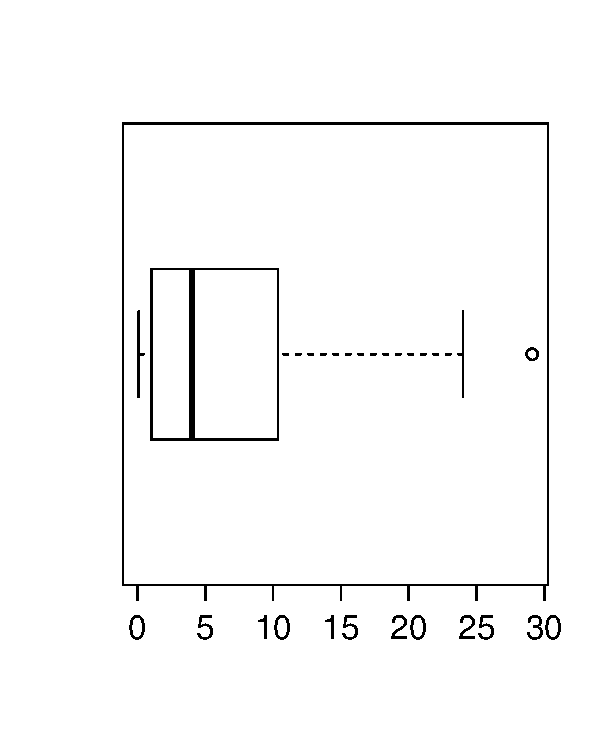
\includegraphics[scale=0.5]{Week3-Q2}

(d) 
%If the new data set (without the outlier) is 
%$\{ y \}$, then we have 
%$\sum_{i=1}^{35} y_{i} = 209$ and $\sum_{i=1}^{35} y_{i}^2 = 2487.04$.

\begin{center}
\begin{tabular}{| l| l| l| l| l|} \hline
 & Mean & Median & Standard deviation & IQR  \\ \hline
Data with largest value $x$ & 6.61 & 4.05 & 7.09 & 9.3 \\  
& & & &  \\  \hline 
Data without largest value $y$ & 5.97 & 4 & 6.04 & 8.85  \\  
& & & &  \\  \hline 
Relative Change (\%) & (6.61-5.97)/6.61 & (4.05 -4)/4.05 & (7.09-6.04)/7.09 & (9.3-8.85)/9.3  \\ 
  & = 9.6 \% & = 1.2 \% & = 14.8 \% &  = 4.8 \% \\ \hline
\end{tabular} 
\end{center}


%Calculations: \\
%$\bar{y} = \frac{209}{35} = 5.97$ \\
%$\tilde{y} = x_{(18)} = 4$ \\
%$s_{y}= \sqrt { \frac{1}{34}\left( 2487.04 - \frac{1}{35} (209)^2\right) } \approx 6.04$ \\
%$s_{y}^2 \approx 36.44$ \\
%$Q_{1} = \frac{1.0 + 1.1}{2} = 1.05$ \\
%$Q_{3} =  \frac{9.9+9.9}{2}  = 9.9 $ \\
%$IQR = 9.9-1.05 = 8.85$. \\

\vspace{.5cm}
(e) 
Comment: Notice that the median and IQR have small relative change compared to the mean and sd, as they are robust.
\end{solution}



\newpage
\hspace{-1cm} {\bf Extra Questions}

\question Comparison of Boxplots \\

Students completed an online quiz consisting of 20 questions, resulting in the following marks.

\begin{center}
Students who had Studied (A): 9 10 11 12 12 13 14 15 15 16 17 17 18 \\
Students who had not studied (B): 1 3 5 8 9 9 10 10 12 12 14 15 16
\end{center}

\begin{parts}
\part  By hand, produce boxplots for A and B.  \\

\part  Produce the boxplots in R. 

\begin{knitrout}
\definecolor{shadecolor}{rgb}{0.969, 0.969, 0.969}\color{fgcolor}\begin{kframe}
\begin{alltt}
\hlstd{a}\hlkwb{=}\hlkwd{c}\hlstd{(}\hlnum{9}\hlstd{,}\hlnum{10}\hlstd{,}\hlnum{11}\hlstd{,}\hlnum{12}\hlstd{,}\hlnum{12}\hlstd{,}\hlnum{13}\hlstd{,}\hlnum{14}\hlstd{,}\hlnum{15}\hlstd{,}\hlnum{15}\hlstd{,}\hlnum{16}\hlstd{,}\hlnum{17}\hlstd{,}\hlnum{17}\hlstd{,}\hlnum{18}\hlstd{)}
\hlstd{b}\hlkwb{=}\hlkwd{c}\hlstd{(}\hlnum{1}\hlstd{,}\hlnum{3}\hlstd{,}\hlnum{5}\hlstd{,}\hlnum{8}\hlstd{,}\hlnum{9}\hlstd{,}\hlnum{9}\hlstd{,}\hlnum{10}\hlstd{,}\hlnum{10}\hlstd{,}\hlnum{12}\hlstd{,}\hlnum{12}\hlstd{,}\hlnum{14}\hlstd{,}\hlnum{15}\hlstd{,}\hlnum{16}\hlstd{)}
\hlkwd{boxplot}\hlstd{(a,b)}
\hlkwd{boxplot}\hlstd{(a,b,} \hlkwc{horizontal}\hlstd{=}\hlnum{TRUE}\hlstd{,}\hlkwc{col}\hlstd{=}\hlkwd{c}\hlstd{(}\hlstr{"green"}\hlstd{,}\hlstr{"blue"}\hlstd{))}    \hlcom{# More colourful version!}
\end{alltt}
\end{kframe}
\end{knitrout}

\vspace{.2cm}
\part Comment on your findings.

\end{parts}


\begin{solution}
(a) \\

For A: \\
$\tilde{x} = x_{(7)} = 14$ \\
$Q_{1} = x_{(4)} = 12 $ \\
$Q_{3} =  x_{(10)} = 16 $ \\
$IQR = 16-12 = 4$ \\
$LT = Q_{1} - 1.5*IQR = 12-6 = 6$ \\
$UT = Q_{3} + 1.5*IQR = 16+ 6 = 22$ \\
Comparing to sorted data, we see there are no data points outside LT and UT, hence there are no outliers.\\

For B: \\
$\tilde{x} = x_{(7)} = 10$ \\
$Q_{1} = x_{(4)} = 8 $ \\
$Q_{3} =  x_{(10)} = 12 $ \\
$IQR = 12-8 = 4$ \\
$LT = Q_{1} - 1.5*IQR = 8-6 = 2$ \\
$UT = Q_{3} + 1.5*IQR = 12+ 6 = 18$ \\

Comparing to sorted data, we see there is one data point lower than LT, hence there is one outlier at 1.\\

Check quartiles in R:
\begin{knitrout}
\definecolor{shadecolor}{rgb}{0.969, 0.969, 0.969}\color{fgcolor}\begin{kframe}
\begin{alltt}
\hlkwd{fivenum}\hlstd{(a)}
\hlkwd{fivenum}\hlstd{(b)}
\end{alltt}
\end{kframe}
\end{knitrout}

Check your 2 boxpots against output in (b).  \\

(c) 
Comments: The students who hadn't studied (B) have a lower median and a much bigger spread of marks than the students who had studied (A).  One student in B has a mark (1) which is much lower than the whole rest of cohort.

\end{solution}



\question Mean and median \\

\begin{parts}
\part The sample average age of 5 people in a room is 30 years.  A 36 year old person walks into the room. Now what is the average age of the people in the room? 

\part Suppose the median age is 30 years and a 36 year old person enters the room. Can you find the new median age from this information?
\end{parts}
		
\begin{solution}
Let $x_i$ denote the $i^{th}$ person in the room. Initially there are 5 people in the room:
$\bar{x} =\frac{1}{5}\displaystyle\sum_{i=1}^5 x_i = 30$.
Hence the sum of the ages of the 5 people is $\displaystyle\sum_{i=1}^5 x_i =150$. \\

When person 6 enters the room 
the sum of the ages is $\displaystyle\sum_{i=1}^6 x_i =150+36$. Thus the new mean age will be
$\bar{x}=\frac{1}{6}\displaystyle\sum_{i=1}^6 x_i = 31$. 

\vspace{.5cm}
Order the individuals by age, initially we can deduce that $x_{(3)}=30$ by the median. When person 6 enters the room the median will now be $Q_2=\frac{x_{(3)}+x_{(4)}}{2}$, as there is no 
way to determine $x_{(4)} $ we can not deduce the new median age.
\end{solution}



\question (Extension: Sigma Notation) \\

Show that the 3 formulae for variance are equal.

\begin{solution}
\begin{align*}
s^2  & = \frac{1}{n-1}  \sum_{i=1}^n  (x_{i} -\overline{x} )^{2}      \\
 &= \frac{1}{n-1}  \left(     \sum_{i=1}^n  x_{i} ^2   +  \sum_{i=1}^n \overline{x}^2 - 2 \sum_{i}^n x_{i}\overline{x} \right)   \\
&= \frac{1}{n-1}  \left(     \sum_{i=1}^n  x_{i} ^2   +  n \overline{x}^2 - 2\overline{x} \sum_{i}^n x_{i} \right)   \\
&= \frac{1}{n-1}  \left(     \sum_{i=1}^n  x_{i} ^2   +  n \overline{x}^2 - 2\overline{x}    n \frac{\sum_{i}^n x_{i} }{n}    \right) \\
&= \frac{1}{n-1}  \left(     \sum_{i=1}^n  x_{i} ^2   +  n \overline{x}^2 - 2\overline{x}    n \overline{x}    \right)   \\
&= \frac{1}{n-1}  \left(     \sum_{i=1}^n  x_{i} ^2   +  n \overline{x}^2 - 2n\overline{x}^2       \right)   \\
&= \frac{1}{n-1}  \left(     \sum_{i=1}^n  x_{i} ^2   -  n \overline{x}^2 \right) \nonumber  \\
&= \frac{1}{n-1}  \left(     \sum_{i=1}^n  x_{i} ^2   -  n \left (\frac{\sum_{i=1}^{n} x_{i} }{n} \right)^2   \right)   \\
&= \frac{1}{n-1}  \left(     \sum_{i=1}^n  x_{i} ^2   -  \frac{1}{n} \left (\sum_{i=1}^{n} x_{i} \right)^2   \right)   \\
\end{align*}
\end{solution}
\end{questions}
\end{tutorial}
\end{document}

